% !TeX root = ../main.tex
\chapter{Introduction}\label{chapter:introduction}

\section{Motivation}\label{section:motivation}

\begin{sloppypar}%
  \ac{VR} is an emerging technology, which provides new ways to present and interact with digital information. Best practices are not yet defined, which leaves much room for new methods and research. Viewing \ac{3D} \acp{VE} using a \ac{VR} headset (or \ac{HMD}) is a great experience. But \ac{VR} shines when interactivity comes into play. Since consumer \acp{HMD} are now available, the development of consumer tracked hand controllers (also known as \ac{VR}/\ac{3D}/hand/motion controllers) has begun. By mapping the \enquote{interaction devices} of the human body to a \ac{VE}, the user is given a natural way of controlling and interacting with the virtual world. While common consumer \ac{VR} headsets are rather similar to each other, motion controllers differ a lot from each other, as seen in Figure~\ref{fig:vr-controllers}.
\end{sloppypar}%

\begin{figure}[H]%
  \centering%
  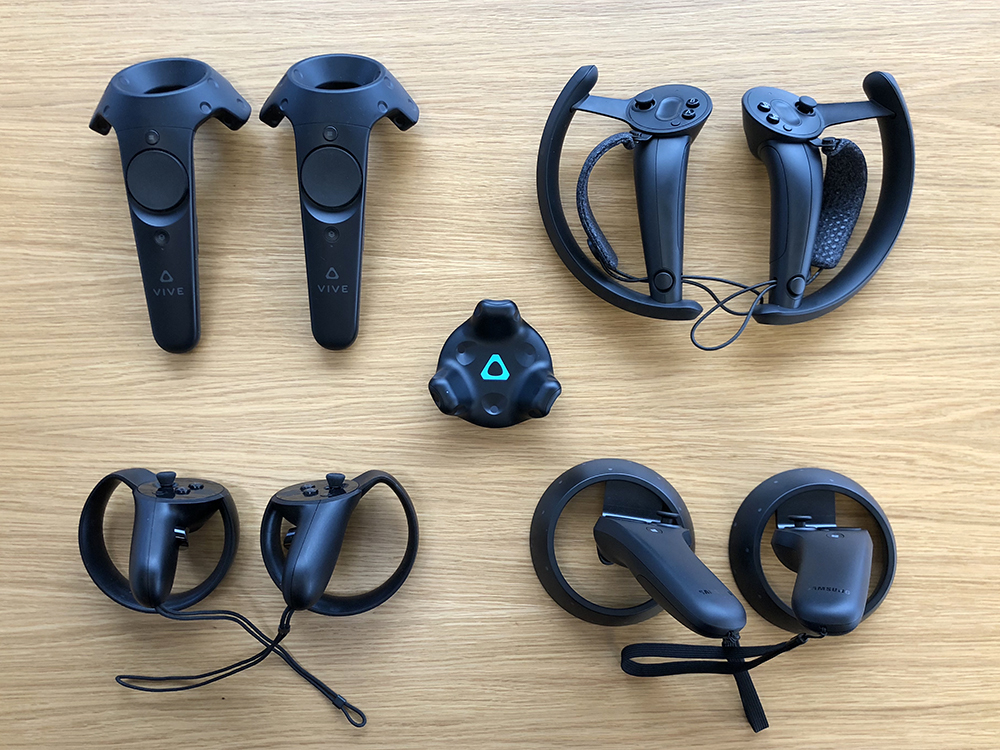
\includegraphics[width=9cm]{figures/introduction/vr_controllers.jpg}%
  \caption[Collection of VR controllers]{A collection of different \ac{VR} controllers. From left to right, top to bottom: HTC VIVE Controllers, Valve Index Controllers (\enquote{Knuckles}), VIVE Tracker, Oculus Touch Controllers, Samsung Odyssey Controllers.\source{Lawrence Yang, \href{https://steamcommunity.com/games/250820/announcements/detail/1697188096865619876}{www.steamcommunity.com/games/\dots/announcements/\dots}}}\label{fig:vr-controllers}
\end{figure}

As of now, most controllers try to map the movement of our real fingers to the virtual world. The Leap Motion\footnote{The Leap Motion controller is a hand tracking device, which is often used to display a hand avatar. Website: \href{https://www.leapmotion.com/}{www.leapmotion.com}} sensor uses multiple infrared cameras to track hand poses, which is only possible in front of the sensor. Newer generations of \ac{VR} controllers do this, too. The Oculus Touch\footnote{The Oculus Touch controllers are hand tracking devices included with the Oculus Rift \ac{HMD}. Website: \href{https://www.oculus.com/rift/}{www.oculus.com/rift}} controllers track the distance of the fingers from the controller and the Valve Index\footnote{The Valve Index is a \ac{HMD} which includes its own set of controllers, called \enquote{Knuckles}. Website: \href{https://store.steampowered.com/valveindex}{store.steampowered.com/valveindex}} controllers even have pressure sensors built-in.
However, for many interactions, hand inspired controllers are not ideal. This applies especially to productive \ac{VR} applications, which require interactions like inputting text for labeling. Since conventional \ac{VR} controllers are designed for some specific tasks (like hand movements), they are tedious to use for other tasks. They also require complex tracking systems. 

The Google Cardboard\footnote{The Google Cardboard is a \ac{HMD} made out of cardboard, which uses a smartphone as a display and for tracking. Website: \href{https://vr.google.com/cardboard/}{vr.google.com/cardboard}} uses a smartphone as a display and for tracking. This makes it an inexpensive \ac{VR} headset, but also demonstrates the versatility of a smartphone. Most people already have a smartphone, since they are general-purpose devices and not very expensive anymore. Thanks to \ac{WLAN} and Bluetooth\footnote{Bluetooth is a wireless standard for exchanging data over short ranges between mobile devices.} it is easy to connect the smartphone to other devices. They have input devices like buttons, a touch screen as well as sensors and systems like a \ac{IMU}\footnote{An IMU is an electronic component which is part of most smartphones and allows to measure a specific force, angular rate, and magnetic field.}. Also, output devices like vibration motors and speakers are present. This makes them similar to \ac{VR} controllers. 

One significant difference between smartphones and common \ac{VR} controllers is that smartphones do not have positional tracking built-in. The position can be estimated using an \ac{IMU}, but since the error accumulates over time, other tracking methods have to be used to correct the drift~\cite{Zhang.2015}. Sophisticated approaches using the phone camera are computationally expensive and still not as good as complete tracking systems.
Besides the missing positional tracking, the advantages lead to the assumption that the smartphone can be used as an alternative \ac{VR} controller. 


\section{Problem Statement}\label{section:problem-statement}
This thesis aims to explore the possibilities of using the smartphone as an interaction device in \ac{VR} experiences. Different methods of implementing the phone as an alternative input device for typical \ac{VR} interactions are going to be presented and evaluated. They are going to be implemented in experiments using the \ac{UBII} architecture, to create an abstracted and reusable system. The goal of those experiments is not to create a better system, but rather show that the smartphone can be used as well as common \ac{VR} controllers for certain interactions. Additional tasks, to complete in the experiments, are going to be implemented to evaluate the presented methods in a usability study.


\section{Outline}\label{section:outline}
In the next chapter, previous work on this topic is presented. Before discussing the implementation of the experiments in the following chapter, \ac{UBII} and the technology used to make the experiments possible, is introduced. The user study and its approach are presented afterward. After discussing the results of the study, the conclusion is drawn.